%% main.tex — v10.0 REFRAMED for a general finance readership (title option B)
%% Alan hard rules (see FACT):
%%   - line numbers NOT loaded (uncomment two lines below on R&R only)
%%   - table captions ABOVE
%%   - American English (analyze/color/harmonize)
%%   - single author: Hongjun Gou @ ICBC Beijing 100140
%%
%% REFRAMING (v10.0, authorised by Alan 20261023 after three desk rejects):
%%   The 20260828 title/abstract freeze is lifted for this variant only.
%%   Title drops "The Geometry of ... as Virtual Fundamental Classes";
%%   the abstract now leads with the stablecoin basket-risk problem and the
%%   supervisory diagnostic, and the virtual-fundamental-class apparatus is
%%   presented as the structural prior that delivers the result rather than
%%   as the paper's identity. Body sections 2-6 are unchanged.
%%   The frozen-framing version remains available as v9.0 (and v6.0-v8.0).
\documentclass[12pt,article]{article}
\usepackage[margin=1.25in]{geometry}
\usepackage[T1]{fontenc}
\usepackage[utf8]{inputenc}
\usepackage{lmodern}
\usepackage{amsmath,amssymb,amsthm,mathrsfs,mathtools}
\usepackage{graphicx}
\usepackage[svgnames,table]{xcolor}
\usepackage[colorlinks=true,linkcolor=black,citecolor=black,urlcolor=black]{hyperref}
\usepackage{booktabs}
\usepackage{array}
\usepackage{setspace}
\usepackage{titling}
\usepackage{titlesec}
\usepackage[round,authoryear]{natbib}
\usepackage{float}
\usepackage[section]{placeins}  %% \FloatBarrier and per-section barrier
\usepackage{enumitem}
%\usepackage{lineno}   %% uncomment on R&R
%\linenumbers          %% uncomment on R&R

\onehalfspacing
\setcounter{secnumdepth}{3}

\newtheorem{theorem}{Theorem}
\newtheorem{proposition}[theorem]{Proposition}
\newtheorem{corollary}[theorem]{Corollary}
\newtheorem{lemma}[theorem]{Lemma}
\theoremstyle{definition}
\newtheorem{definition}[theorem]{Definition}
\newtheorem{assumption}[theorem]{Assumption}
\newtheorem{remark}[theorem]{Remark}

\DeclareMathOperator{\rk}{rk}
\DeclareMathOperator{\coker}{coker}
\newcommand{\Mconf}{\mathcal{M}}            %% ambient configuration moduli (carries the VFC)
\newcommand{\Mpeg}{\mathcal{M}_{\mathrm{peg}}} %% peg-preserving locus inside \Mconf
\newcommand{\Bpeg}{\mathcal{B}}
\newcommand{\Wpeg}{\mathcal{W}}
\newcommand{\Sigmait}{\Sigma}
\newcommand{\Covit}{C}          %% co-movement covariance (carries the rank-one wall jump)
\newcommand{\Deltait}{\Delta}   %% induced jump (covariance, or its normalised correlation image)
\newcommand{\Lambdait}{\Lambda} %% retained for the appendix
\newcommand{\Omit}{\Omega}
%% AUTOGENERATED by scripts/inject_numbers.py — do not edit by hand.
\newcommand{\NPANEL}{28}
\newcommand{\NEVENTS}{9}

%% AUTOGENERATED by scripts/estimator_gradient.py — do not edit by hand.
\newcommand{\GFDUSDB}{-0.0762}
\newcommand{\GFDUSDC}{0.0838}
\newcommand{\GFDUSDDID}{-0.2464}
\newcommand{\GFDUSDHI}{-0.0921}
\newcommand{\GFDUSDLO}{-0.3705}
\newcommand{\GFDUSDNB}{1}
\newcommand{\GFDUSDNC}{44}
\newcommand{\GFDUSDNO}{231}
\newcommand{\GFDUSDO}{0.1867}
\newcommand{\GFDUSDPCOIN}{0.7671}
\newcommand{\GFDUSDPCT}{23.3}
\newcommand{\GFDUSDPPAIR}{0.7593}
\newcommand{\GFTXB}{0.4937}
\newcommand{\GFTXC}{-0.1404}
\newcommand{\GFTXDID}{0.5130}
\newcommand{\GFTXHI}{0.6555}
\newcommand{\GFTXLO}{0.4101}
\newcommand{\GFTXNB}{1}
\newcommand{\GFTXNC}{32}
\newcommand{\GFTXNO}{120}
\newcommand{\GFTXO}{0.0130}
\newcommand{\GFTXPCOIN}{0.1553}
\newcommand{\GFTXPCT}{84.5}
\newcommand{\GFTXPPAIR}{0.1581}
\newcommand{\GUSDCSVBB}{0.9970}
\newcommand{\GUSDCSVBC}{0.4219}
\newcommand{\GUSDCSVBDID}{0.6871}
\newcommand{\GUSDCSVBHI}{1.0065}
\newcommand{\GUSDCSVBLO}{0.3754}
\newcommand{\GUSDCSVBNB}{3}
\newcommand{\GUSDCSVBNC}{45}
\newcommand{\GUSDCSVBNO}{105}
\newcommand{\GUSDCSVBO}{0.2619}
\newcommand{\GUSDCSVBPCOIN}{0.0109}
\newcommand{\GUSDCSVBPCT}{98.9}
\newcommand{\GUSDCSVBPPAIR}{0.0025}
\newcommand{\GUSDCSVBPURE}{1.1849}
\newcommand{\GUSDCSVBPUREN}{1}


\newif\ifanon
\ifdefined\ANONBUILD\anontrue\fi

\title{\Large Correlation Rigidity and Contagion in Stablecoin Baskets:\\[2pt]
\Large A Structural Diagnostic for Supervisors}
\ifanon
  \author{}
\else
  \author{Hongjun Gou\thanks{Industrial and Commercial Bank of China, Beijing 100140, China. Email: \texttt{gouhongjun\_bs@cq.icbc.com.cn}.}}
\fi
\date{}

\begin{document}
\maketitle

\begin{abstract}
US-dollar stablecoins now form a systemic layer of crypto finance; basket margin, index perpetuals and proof-of-reserves price one unobservable object, the joint peg-deviation correlation surface of a basket. Typically only three or four deviate, and published correlations are smoothed across the gaps. We posit that the gaps are structural rather than noise: co-movement is rigid within a regime and jumps across its boundary, at eight stress boundaries, one per failure channel. Basket risk is a staircase, not a slope. Every locally continuous estimator must forgo that jump. A supervisor can run the diagnostic on public prices alone: on the USDC--SVB weekend the co-movement jump is concentrated on the coins that shared the failing custodian, and the largest jump of all falls on a pair excluding the coin that broke.

\medskip
\noindent\textbf{Keywords:} stablecoins; de-peg contagion; correlation rigidity; wall-crossing; basket pricing; regime switching.

\medskip
\noindent\textbf{JEL classification:} G12; G23; C58; C65.
\end{abstract}


\section{Introduction}\label{sec:intro}
The market for US-dollar stablecoins has grown into a systemic layer of the crypto financial system, with basket-margin arrangements at centralized exchanges, index perpetuals on decentralized venues, and proof-of-reserves frameworks at regulated issuers all depending on the same object: a joint de-peg correlation surface that no market participant has ever actually observed---on a representative day, only three or four coins in a basket exhibit any peg deviation at all, and the correlation matrices published by clearinghouses, index providers, and regulators are filled in by smoothing over the gaps. The trouble is that the gaps are not statistical noise around a densely sampled surface; they are \emph{structural discontinuities}, and a smoother that cannot see the discontinuities systematically understates the joint tail risk it is meant to price.

Two edges of the same question follow. What is the sharpest description any correlation model can produce of the joint de-peg behavior that a stablecoin basket actually exhibits, as opposed to the smooth surface that basket-margin frameworks assume? And what is the intrinsic information content of a constraint variety on which peg-preserving equilibria fail on codimension-one strata organized by structural cause? The economic edge and the mathematical edge, it turns out, admit a common answer. That answer identifies a market-specific ceiling on what any smooth-surface method can achieve---a \emph{correlation-rigidity ceiling}\footnote{The notion of \emph{correlation rigidity} used here is structural---the local constancy of the co-movement structure within a regime, and its failure across a regime boundary---not the risk-management sense of ``rigid correlation matrix'' in \citet{Li2000} and the copula-parametric literature that follows it.}---and identifying its location is the object of this paper.

Three literatures speak to the question and none has resolved it. Stablecoin economics---the money-view foundations of \citet{GortonEtal2022, CatalinKirk2022}, empirical stability channels of \citet{LyonsViswanath2023, dAvernasEtal2024}, run dynamics of \citet{MaZengZhang2023}, noncustodial stability of \citet{Klages2022, KlagesMundtMinca2020}, general-equilibrium \citep{RoutledgeZetlin2022}, Terra analyses \citep{Uhlig2022, LiuLiSprenger2023}, and policy overlays \citep{FSB2023Stablecoin, BIS2023Stablecoin, PWG2021Stablecoin}---takes the peg-deviation process as given and studies its stability at the single-name level, not the cross-sectional correlation object that basket-margin rules price. Correlation baselines---Gaussian copula \citep{Li2000}, Vasicek single-factor \citep{Vasicek2002}, regime-switching \citep{Pelletier2006}, dynamic equicorrelation \citep{EngleKelly2012}, POET \citep{FanLiaoMincheva2013}, shrinkage \citep{LedoitWolf2004}, with the structural critique of \citet{CovalJurekStafford2009} and asymmetric-crisis evidence of \citet{AngChen2002}---impose a smooth correlation surface on a parametric family and do not bound how sharply correlation can be recovered when the constraint variety is naturally singular. Orthogonal to these, an implicit-atlas programme of virtual fundamental classes \citep{FukayaOno1999, LiTian1998, BehrendFantechi1997, Pardon2016, Pardon2019}, the wall-crossing formalism of \citet{KontsevichSoibelman2008, Bridgeland2007}, and the derived-critical-locus bridge of \citet{Joyce2015} produced the sharpest foundations for enumerative invariants on constraint varieties with codimension-one singular strata; to the author's knowledge, no prior work applies implicit-atlas VFCs to a financial-economic object.

Closing the gap requires an object that lives natively in both worlds. This paper represents the stablecoin issuer configuration as a point of a configuration space $\Mconf$ (\S\ref{sec:moduli}), whose peg-preserving locus is cut out by the peg constraint and whose strata are indexed by failure channel---backing-ratio, oracle, redemption, custody, bridge, regulatory, funding-rate, interest-rate. Across the boundary of a stratum the joint co-movement structure jumps by a rank-one term supported on the affected coins, and no smooth surface can reproduce that jump. The residue is stated on the co-movement \emph{covariance}, not on the correlation matrix, and the choice is forced rather than stylistic: a rank-one additive jump supported on a block of two or more coins necessarily adds a positive amount to its own diagonal, which a correlation matrix cannot absorb on either chamber side, since its diagonal is fixed at one. Carrying the crossing law on the covariance and passing to correlations by the normalising map removes the obstruction exactly, because that map \emph{assigns} the unit diagonal rather than computing it. Within a chamber of the peg-preserving parameter space, co-movement is locally constant and insensitive to smooth deformation of issuance rules; across a wall it jumps, and the jump has a closed form we state rather than estimate. Read economically, the three steps buy a single testable implication: the jump is \emph{supported on a small block of coins}, with a sign fixed by the wall taxonomy before the event window is observed, and it survives normalisation as a signed three-tier footprint on the correlation matrix rather than as a rank-one object. We call this footprint the \emph{block signature} of the wall---the coin pairs whose co-movement moves, and the sign in which it moves. This is the sense in which we use the word \emph{contagion}: not a diffuse rise in co-movement across the whole market, but a structured rise confined to the coins a failure channel touches, which is exactly what makes it identifiable. The block signature is what a supervisor reads off an acute-window correlation submatrix, and it is what every smooth-surface method is structurally unable to place there. That is what makes the diagnostic falsifiable rather than fitted.

The paper's diagnostic---basket risk is a staircase, not a slope---rests on three parallel contributions.

\textit{First, a structural representation of basket risk with a wall-stratified parameter space.} We represent the joint peg-preserving equilibrium as a configuration space---a parameter space whose geometry is inherited from the constraint that every issuer keep its peg---so that the stress boundaries unique to markets with structurally distinct failure triggers appear as strata rather than as features to be estimated. The construction reads directly off any public stablecoin panel and turns a two-dimensional smoothing exercise into a stratified recovery problem.

\textit{Second, a rigidity-and-crossing framework whose consequences are made explicit.} Three properties are posited and their consequences proved. The properties: co-movement constant within a failure regime up to a positive scale; a jump across a regime boundary that is a signed sum of rank-one terms; and support of that jump on the coins the boundary's channel touches. The consequences: correlation rigidity on chambers, with the scale cancelled exactly, so that rigidity survives normalisation without a further assumption; zero diagonal for the induced correlation jump; a signed three-tier footprint on the correlation image, replacing the rank-one structure that the normalisation destroys; and the gap $\pm\tfrac12\Deltait_R$ separating the true correlation from any locally continuous surface. Together these are what make basket risk a staircase rather than a slope---the question is not what the surface does between boundaries, because on a chamber it does nothing---and the passage to correlations tells us exactly what part of the block signature an estimator could even in principle target.

\textit{Third, a pair-level test of the block prediction.} Because the normalisation destroys rank-one structure and leaves a signed footprint, the empirical object is a gradient across pair layers: pairs of coins both inside the wall-affected block move up, pairs with one coin inside move the other way, and pairs with neither do not move at all. The block-versus-rest contrast differences out the crisis-wide co-movement that raises every layer at once. On a nine-event 2020--2025 panel built entirely from public data, the USDC--SVB custody event delivers the predicted block effect, with a block-versus-rest contrast of \GUSDCSVBDID\ and a coin-level permutation $p = \GUSDCSVBPCOIN$; the pair $(\text{DAI},\text{FRAX})$, which contains neither the primary victim nor any coin with direct custody exposure, jumps by \GUSDCSVBPURE---the largest of any pair---so the gradient is a block effect rather than a victim effect. The result survives a full $3\times3$ window grid. The test applies to the three events that carry a multi-coin block. The construction additionally identifies which policy instruments the block signature would key.

The remainder of the paper proceeds as follows. Section~\ref{sec:moduli} defines the stablecoin state, the configuration space and its peg-preserving locus, and states which properties of that space the paper assumes and which it derives. Section~\ref{sec:rigidity} defines co-movement as a second moment, takes the correlation matrix as its normalised image, and proves that rigidity of the covariance yields rigidity of the correlation matrix. Section~\ref{sec:wall} states the crossing law, derives its consequences for correlations, maps the eight stress walls, and contrasts them with the Gaussian copula. Section~\ref{sec:empirical} builds and runs the pair-level gradient test on the nine-event panel. Section~\ref{sec:conclusion} concludes; robustness checks are in the Appendix.


\section{The Peg-Preserving Configuration Space}\label{sec:moduli}
The staircase of the introduction needs an object underneath it. This section defines the state of a stablecoin (\S\ref{sec:tuple}), the space of joint configurations and the locus on which the peg holds (\S\ref{sec:mpeg}), and states plainly which properties of that space the paper assumes and which it derives (\S\ref{sec:what-is-assumed}). The space is not decorative: it is what makes ``which failure channel is stressed'' a coordinate rather than a narrative device, and it is the object the eight stress walls of \S\ref{sec:wall} stratify.

\subsection{Stablecoin state and peg preservation}\label{sec:tuple}
\begin{definition}[Stablecoin state]\label{def:stable}
At a point in time, a stablecoin is a tuple $s_i = (C_i, O_i, R_i)$ where
\begin{itemize}
\item $C_i \in \Delta^{K-1}$ is the collateral composition, a point of the $(K-1)$-simplex over $K$ underlying reserve asset classes (fiat deposits, Treasury bills, corporate paper, crypto-collateral, algorithmic-endogenous);
\item $O_i \in [0.5, 1.5]^J$ is the oracle price vector, a set of $J$ price feeds each reporting the coin's market price in USD, with an oracle-consensus rule $\bar{O}_i = \phi_i(O_i)$;
\item $R_i \in \{\texttt{open}, \texttt{gated}, \texttt{halted}\}$ is the redemption gate state, a discrete label carrying no continuous degree of freedom.
\end{itemize}
Two quantities are derived from the state rather than carried by it. The \emph{signed peg deviation} is $\delta_i := \bar{O}_i - 1$. The \emph{backing ratio} is $\rho_i := \mathrm{value}(C_i)/\mathrm{supply}_i$, which is fixed by the issuer's outstanding supply and is therefore not a free coordinate of $s_i$. Counting continuous degrees of freedom, $s_i$ contributes $(K-1)$ collateral plus $J$ oracle coordinates, i.e.\ $K + J - 1$.

A state is \emph{peg-preserving} at tolerance $\varepsilon$ if $|\delta_i| \le \varepsilon$ and the redemption arbitrage cycle (mint at par $\to$ sell at market $\to$ redeem at par) is executable with round-trip profitability bounded by the same $\varepsilon$. The default threshold $\varepsilon = 50$ basis points is standard \citep{LyonsViswanath2023}. The threshold enters only in the definition of peg preservation, not in the covariance, the crossing law or the test: the empirical section compares acute to pre-event windows and never uses $\varepsilon$ as a cut-off, so no robustness sweep over it is required.
\end{definition}

\begin{remark}[Why peg preservation is stated pointwise]\label{rem:pointwise}
An earlier formulation required $|\bar{O}_i(t) - 1| \le \varepsilon$ for all $t \in [0,T]$. That is a condition on a \emph{trajectory}, and $s_i$ carries no time coordinate, so it could not be evaluated on the objects the configuration space consists of. The definition above is pointwise, and the horizon enters only where it belongs, in the empirical windows of \S\ref{sec:panel}.
\end{remark}

\subsection{The configuration space and the peg-preserving locus}\label{sec:mpeg}
\begin{definition}[Configuration space and its peg-preserving locus]\label{def:mconf}
Fix $N$ stablecoins. The \emph{configuration space} is
\[
\Mconf = \{(s_1,\ldots,s_N) \mid \text{joint feasibility holds}\},
\]
where joint feasibility comprises (i) backing balance, (ii) oracle consistency, and (iii) redemption clearing. The \emph{peg-preserving locus} $\Mpeg \subset \Mconf$ is the subset on which every $s_i$ is peg-preserving in the sense of Definition~\ref{def:stable}.
\end{definition}

\begin{assumption}[Non-emptiness]\label{ass:nonempty}
$\Mconf$ and $\Mpeg$ are non-empty on the parameter range considered.
\end{assumption}

The distinction between $\Mconf$ and $\Mpeg$ matters for what follows. Peg preservation is a \emph{constraint} cutting a locus out of the ambient configuration space, not a restriction on what the ambient space may contain. De-pegging configurations remain points of $\Mconf$; they are simply not points of $\Mpeg$. The chambers and walls of \S\ref{sec:rigidity}--\S\ref{sec:wall} stratify the ambient space.

\subsection{What is assumed and what is derived}\label{sec:what-is-assumed}
Three properties do the work in this paper, and all three are stated as explicit assumptions rather than as theorems: within-chamber rigidity (Assumption~\ref{ass:rigidity}), the rank-one form of the jump across a wall (Assumption~\ref{ass:wallcrossing}), and the support of that jump on the wall-affected block (Assumption~\ref{ass:support}). Everything downstream of them is proved: the zero diagonal of the induced correlation jump (Corollary~\ref{cor:wall-jump}), its three-tier footprint (Remark~\ref{rem:small-cases}), and the gap between the true correlation and any smooth surface (Corollary~\ref{cor:copula-fail}). What the empirical section then does is a separate question, taken up in \S\ref{sec:empirical}, of whether the consequences describe the data.

Stating them as assumptions is a choice about where the paper's weight should sit, and the choice deserves an argument. Each of the three is a statement about the joint distribution of peg deviations that can be inspected on public price data, and none requires a parametric family, a distributional assumption, or issuer-internal data. They are not, however, equally exposed to the test below. Assumptions~\ref{ass:wallcrossing} and~\ref{ass:support} are jointly tested by the block-versus-rest contrast of \S\ref{sec:empirical}, which is what that section measures. Assumption~\ref{ass:rigidity} is not separately tested there: it concerns how co-movement behaves as parameters vary \emph{within} a regime, whereas the event design observes regimes only through the windows on either side of a crossing. The design can therefore speak to the crossing and to its support, not to the flatness. The rank-one form is not an arbitrary choice: \S\ref{sec:wall} records its lineage in the Kontsevich--Soibelman wall-crossing formula \citep{KontsevichSoibelman2008}, which takes a product over the charges whose central charges change sign across a wall and, where it applies, yields exactly a signed sum of rank-one terms on the coins those charges carry. Taking that form as the primitive lets a reader who doubts the lineage evaluate the claim on the data rather than on the analogy, which is the arrangement the empirical section is built to support. What the reader is asked to accept is Assumptions~\ref{ass:rigidity}--\ref{ass:support}, and the empirical section is the accounting of whether they are a good description.


\section{Correlation Rigidity}\label{sec:rigidity}
This section supplies the lower half of the staircase: within a failure regime the joint co-movement structure does not move, and no estimator can do better than flat on it. It defines the co-movement covariance as a second moment and the correlation matrix as its normalised image (\S\ref{sec:vfc-int}), characterizes the peg-preserving parameter space and its chamber decomposition (\S\ref{sec:chambers}), states the rigidity assumption (\S\ref{sec:rigidity-thm}), and derives from it the rigidity of the correlation matrix itself.

\subsection{Co-movement covariance and its normalised image}\label{sec:vfc-int}
Write $\delta = (\delta_1,\ldots,\delta_N)$ for the vector of signed peg deviations of Definition~\ref{def:stable}.

\begin{definition}[Co-movement covariance matrix]\label{def:intensity}
Fix a chamber of the peg-preserving parameter space (\S\ref{sec:chambers}) and let $\mu_\theta$ be the probability law of $\delta$ while the system sits in that chamber at parameter $\theta$. The law is a primitive of the framework rather than the output of a specified stochastic process: no dynamics is written down, and the only properties used below are that $\mu_\theta$ is a probability measure with finite second moments. \S\ref{sec:empirical} estimates it by the empirical distribution of daily peg deviations over an estimation window, which is the sense in which the object below and the object measured there are the same. The \emph{co-movement covariance matrix} is
\[
\Covit_{ij}(\theta) := \operatorname{Cov}_{\mu_\theta}(\delta_i,\delta_j)
= \mathbb{E}_{\mu_\theta}\bigl[(\delta_i - \bar\delta_i)(\delta_j - \bar\delta_j)\bigr], \qquad \bar\delta_i := \mathbb{E}_{\mu_\theta}[\delta_i],
\]
and $\Covit(\theta) := \mathbb{E}_{\mu_\theta}[(\delta - \bar\delta)(\delta - \bar\delta)^\top]$. The centring matters and is not cosmetic: it is what makes $\Covit$ the matrix that the correlation estimates of \S\ref{sec:empirical} actually estimate. A stablecoin that trades persistently below par, such as GHO in \S\ref{sec:walltypes}, has $\bar\delta_i \ne 0$, and an uncentred second moment would not be recovered by any correlation estimate computed on its price series. We therefore take the covariance in the usual centred sense throughout.
\end{definition}

Because $\Covit(\theta)$ is an expectation of the positive semidefinite rank-one matrix $(\delta-\bar\delta)(\delta-\bar\delta)^\top$, it is symmetric and positive semidefinite by construction, and $\Covit_{ii}(\theta)$ is the variance of coin $i$'s peg deviation. No property of the measure beyond its existence as a probability is used.

\begin{definition}[Correlation as the normalised image]\label{def:corr}
On the open set where $\Covit_{ii}(\theta) > 0$ for every $i$, the \emph{co-movement correlation matrix} is
\begin{equation}\label{eq:normalised-corr}
\Sigmait_{ij}(\theta) := \frac{\Covit_{ij}(\theta)}{\sqrt{\Covit_{ii}(\theta)\,\Covit_{jj}(\theta)}},\qquad \Sigmait_{ii}(\theta) := 1,
\end{equation}
equivalently $\Sigmait = D^{-1/2}\Covit D^{-1/2}$ with $D := \operatorname{diag}(\Covit)$. The hypothesis $\Covit_{ii}>0$ is what makes the two forms agree and $D^{-1/2}$ real; it is also what Corollary~\ref{cor:rigidity-corr} below uses.
\end{definition}

\begin{remark}[Why the covariance, and not the correlation, carries the crossing law]\label{rem:why-cov}
The wall-crossing operation of \S\ref{sec:wall} is additive and rank-one. That operation is admissible on $\Covit$ but \emph{not} on a correlation matrix: two correlation matrices both have unit diagonal, so their difference must have zero diagonal, whereas a rank-one update $a\,v v^\top$ supported on a block of two or more coins contributes $a v_i^2 > 0$ to the diagonal of the $i$-th coordinate. Stating the crossing law on $\Covit$ and passing to correlations by \eqref{eq:normalised-corr} removes the obstruction exactly, because the normalising map \emph{assigns} the diagonal instead of computing it and therefore absorbs the diagonal increment identically. What it does \emph{not} do is preserve rank-one structure: the normalising map is a nonlinear congruence, so a rank-one additive law on $\Covit$ does not push forward to a rank-one law on $\Sigmait$. Corollary~\ref{cor:copula-fail} states what does survive.
\end{remark}

\begin{remark}[What a probability measure buys]\label{rem:cov-two-consequences}
Taking $\mu_\theta$ to be a probability measure is a substantive choice, and it is the one that makes the rest of the paper coherent. It delivers positive semidefiniteness and the Cauchy--Schwarz bound $|\Sigmait_{ij}|\le 1$, so that $\Sigmait$ is genuinely a correlation matrix rather than an array that merely resembles one. It makes the second moments $\Covit_{ij}$ estimable from any window in which peg deviations vary, including calm windows in which no coin crosses the de-peg threshold, which is what makes the pre-event windows of \S\ref{sec:empirical} usable at all. And it is exactly the object \S\ref{sec:empirical} computes, by taking $\mu_\theta$ to be the empirical distribution of daily peg deviations over the estimation window: theory and measurement are the same moment, not two objects related by analogy.
\end{remark}

\subsection{Peg-preserving parameter space and chambers}\label{sec:chambers}
\begin{definition}[Wall set and chamber]\label{def:chamber}
Let $\Theta_{\mathrm{peg}}$ denote the parameter range over which Assumption~\ref{ass:nonempty} holds. Its coordinates are the structural parameters---issuance rule, collateral haircut, oracle bandwidth---together with the state functionals $\rho_i(\theta)$ and $\delta_i(\theta)$ through which those parameters act, so that a condition such as $\rho_i=1$ is read as the level set $\{\theta : \rho_i(\theta)=1\}$ and defines a wall in $\Theta_{\mathrm{peg}}$ rather than a single configuration. Let $\Wpeg := \bigcup_{k=1}^{8} W_k \subset \Theta_{\mathrm{peg}}$ be the union of the eight stress boundaries enumerated in \S\ref{sec:walltypes}: backing-ratio, oracle-deviation, redemption-gate, custody, bridge, regulatory, funding-rate, and interest-rate/PSM. A \emph{chamber} is a connected component of $\Theta_{\mathrm{peg}} \setminus \Wpeg$.
\end{definition}

Four of the eight walls are defined by an equality between a continuous parameter and a threshold---$W_1$ (backing ratio), $W_2$ (oracle deviation), $W_7$ (funding basis) and $W_8$ (interest spread)---and are codimension-one hypersurfaces in $\Theta_{\mathrm{peg}}$. The other four are discrete transitions between strata rather than passages through a hypersurface: the redemption-gate flip $W_3$, and the custody, bridge and regulatory events $W_4$--$W_6$. All eight are kept in a single list because the failure channel is the same object of supervision and because the crossing each induces in $\Covit$ has the same rank-one form (Assumption~\ref{ass:wallcrossing}); but the reader should not picture all eight as smooth hypersurfaces, and only the first group can be drawn as boundaries in a continuous parameter plane.

\subsection{The rigidity assumption and its consequence}\label{sec:rigidity-thm}
\begin{assumption}[Within-chamber rigidity, H1]\label{ass:rigidity}
For any two parameter values $\theta, \theta'$ in the same chamber, there is a scalar $\lambda = \lambda(\theta,\theta')>0$ such that
\[
\Covit(\theta) = \lambda(\theta,\theta')\,\Covit(\theta').
\]
That is, the co-movement covariance is constant within a chamber up to a positive scale factor.
\end{assumption}

The scale factor is not idle. It allows the overall level of peg-deviation volatility to drift within a regime---which it plainly does---while the \emph{shape} of the co-movement structure is fixed. The paper therefore does not claim that co-movement is numerically frozen; it claims that its proportionality structure is.

\begin{theorem}[Correlation rigidity]\label{thm:rigidity}
Under Assumption~\ref{ass:rigidity}, the correlation matrix $\Sigmait(\theta)$ of \eqref{eq:normalised-corr} is constant on chambers: $\Sigmait(\theta) = \Sigmait(\theta')$ whenever $\theta$ and $\theta'$ lie in the same chamber.
\end{theorem}
\begin{proof}
Fix a chamber and let $\theta,\theta'$ be in it, with $\Covit(\theta) = \lambda\Covit(\theta')$ and $\lambda>0$. Since $\Covit$ is positive semidefinite with $\Covit_{ii}>0$ on the domain of \eqref{eq:normalised-corr}, we have $D(\theta) = \lambda D(\theta')$ and hence $D(\theta)^{-1/2} = \lambda^{-1/2}D(\theta')^{-1/2}$. Therefore
\[
\Sigmait(\theta) = D(\theta)^{-1/2}\Covit(\theta)D(\theta)^{-1/2}
= \bigl(\lambda^{-1/2}D(\theta')^{-1/2}\bigr)\bigl(\lambda\Covit(\theta')\bigr)\bigl(\lambda^{-1/2}D(\theta')^{-1/2}\bigr)
= D(\theta')^{-1/2}\Covit(\theta')D(\theta')^{-1/2} = \Sigmait(\theta'),
\]
the two factors of $\lambda^{-1/2}$ cancelling the $\lambda$. Hence $\Sigmait$ is constant on the chamber.
\end{proof}

\begin{corollary}[Rigidity is inherited, not assumed, at the level of correlations]\label{cor:rigidity-corr}
Theorem~\ref{thm:rigidity} is not a restatement of Assumption~\ref{ass:rigidity}. The assumption is made on $\Covit$ and involves a free scale; the conclusion is a statement about $\Sigmait$ and involves no scale. The normalising map removes the one degree of freedom the assumption leaves open.
\end{corollary}

Corollary~\ref{cor:rigidity-corr} is the \emph{correlation rigidity} of the title: within a regime the joint de-peg correlation matrix of a stablecoin basket does not move, and it is insensitive to the haircut, oracle bandwidth, or issuance rule that vary smoothly inside that regime. Rigidity is the lower step of the staircase; the upper step is the jump of \S\ref{sec:wall}.

\begin{remark}[Economic reading]\label{rem:economic}
Within any regime the cross-sectional correlation structure is determined by which failure channels are latent, not by the specific haircut, oracle bandwidth, or issuance rule in force. This is a moduli-theoretic reading of the empirical rigidity long noted in credit derivatives \citep{CovalJurekStafford2009}. Transitions between regimes require the accounting of \S\ref{sec:wall}.
\end{remark}


\section{Wall-Crossing at Stress Boundaries}\label{sec:wall}
Eight stress-boundary wall types partition $\Theta_{\mathrm{peg}}$ (\S\ref{sec:walltypes}). Across each wall the co-movement covariance jumps by a rank-one term supported on the affected coins (Assumption~\ref{ass:wallcrossing}), and the correlation matrix inherits that jump through the normalising map of \S\ref{sec:rigidity}. This section states the assumption, derives its consequences for correlations, and maps the eight historical de-peg episodes of 2020--2025 onto the wall types (\S\ref{sec:ninewalls}).

\subsection{Wall types}\label{sec:walltypes}
Four of the eight walls are equalities between a continuous structural parameter and a threshold ($W_1$, $W_2$, $W_7$, $W_8$); the other four are discrete transitions ($W_3$--$W_6$). \S\ref{sec:chambers} records why both kinds are kept in one list.
\begin{itemize}[leftmargin=1.8em]
\item[$W_1$] \emph{Backing-ratio}: $\rho_i = 1$; redemption arbitrage fails to clear at par (canonical: DAI, 12 March 2020).
\item[$W_2$] \emph{Oracle-deviation}: $|O_i - 1| = \delta_*$ at the halt threshold (canonical: FDUSD, mid-2024).
\item[$W_3$] \emph{Redemption-gate}: gate flips \texttt{open}$\to$\texttt{gated/halted} at a queue-depth threshold (canonical: UST May 2022; USDT July 2022).
\item[$W_4$] \emph{Custody}: custodian solvency event. Sub-types $W_4$-\texttt{bank} (regulated-bank; canonical: USDC/SVB, 11 March 2023) and $W_4$-\texttt{cex} (CEX/crypto custodian; canonical: FTX contagion, 08--14 November 2022).
\item[$W_5$] \emph{Bridge}: cross-chain bridge exploit/freeze isolates supply (canonical: second-order episodes on wrapped stablecoins).
\item[$W_6$] \emph{Regulatory}: regulator-forced wind-down / freeze (canonical: NY DFS $\to$ Paxos/BUSD, February 2023).
\item[$W_7$] \emph{Funding-rate}: delta-neutral synthetic issuer's perpetual-basis sign/magnitude change stresses the peg-arbitrage cycle (canonical: USDe, April--May 2024; max daily deviation $59$ bp on 2024-05-02---a marginal threshold crossing at the boundary $\varepsilon = 50$ bp). We record $W_7$ as a threshold-crossing wall of low peg-deviation intensity; the wall taxonomy applies to the local (small-signal) regime, and the amplitude of the rank-one lift of Assumption~\ref{ass:wallcrossing} is attenuated as the deviation approaches the threshold from above.
\item[$W_8$] \emph{Interest-rate / PSM}: interest-rate-driven coin with PSM buffer holds structural sub-peg when spread does not clear the buffer (canonical: GHO, 18 December 2024, closing price \$0.8085 on DeFiLlama daily snapshot, i.e., $\approx 19\%$ sub-peg).
\end{itemize}

Figure~\ref{fig:wall} illustrates the resulting chamber/wall geometry on the two continuous coordinates $(\rho, \delta)$ that carry $W_1$ and $W_2$; discrete walls $W_3$--$W_6, W_8$ appear as external annotations, and the funding-rate wall $W_7$, being one-sided in the basis, is absorbed into the boundary behavior of the $\rho$ axis.

\begin{figure}[H]
\centering
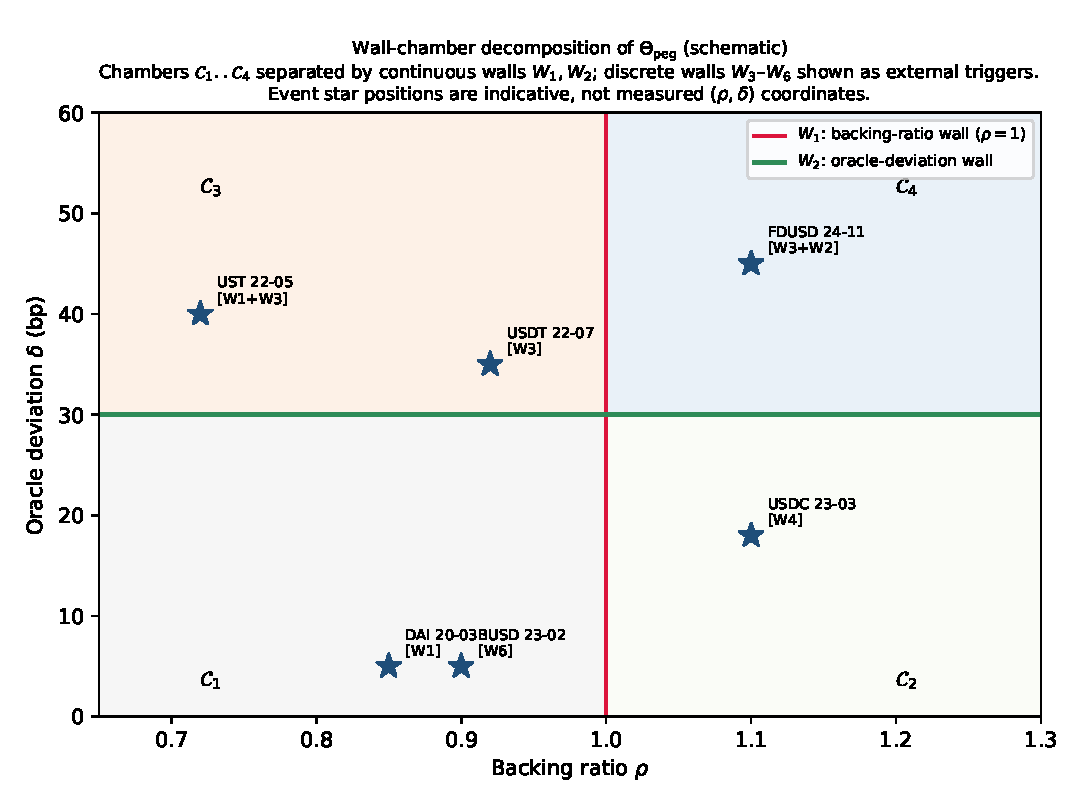
\includegraphics[width=0.78\textwidth]{figs/fig1_wall_chamber}
\caption{Wall-chamber decomposition of the peg-preserving parameter space $\Theta_{\mathrm{peg}}$ projected to the $(\rho, \delta)$-plane, drawn as a schematic illustration of the chamber/wall geometry. Continuous walls $W_1$ (backing-ratio, red) and $W_2$ (oracle-deviation, green) carve out four smooth chambers in this projection; the discrete triggers $W_3$--$W_6$ are annotated as external events, and the two further continuous walls $W_7$ and $W_8$ act on coordinates outside the $(\rho,\delta)$ plane and are not drawn.}
\label{fig:wall}
\end{figure}

\subsection{The crossing law}\label{sec:ks}
\begin{assumption}[Rank-one wall crossing, H2]\label{ass:wallcrossing}
Fix a wall $W \subset \Wpeg$ separating two adjacent chambers, and write $\Covit^\mp := \Covit(\theta^\mp)$ for the co-movement covariance matrices of Definition~\ref{def:intensity} on the two sides. Then
\begin{equation}\label{eq:wall-crossing}
\Covit^+ - \Covit^- = \sigma_W \sum_{\gamma \in \Gamma_W} \Omit(\gamma) \, v_\gamma v_\gamma^\top ,
\end{equation}
where $\Gamma_W$ is a finite index set of \emph{de-peg channels} active at $W$, $\Omit(\gamma) \in \mathbb{R}$ is a signed weight attached to channel $\gamma$, $v_\gamma \in \mathbb{R}^N$ is a direction vector supported on the coins that channel $\gamma$ affects, and $\sigma_W > 0$ is a single positive scalar amplitude.
\end{assumption}

\begin{assumption}[Block support, H3]\label{ass:support}
For each wall $W$ crossed by an episode with a multi-coin failure channel, the directions $\{v_\gamma\}_{\gamma \in \Gamma_W}$ span the indicator directions of a single group of coins $B_W$, the \emph{wall-affected block}: the coins that share the failing custodian, the crossing oracle, or the gating issuer as the case may be. Coins outside $B_W$ carry zero weight.
\end{assumption}

The shape of \eqref{eq:wall-crossing} is the shape of the Kontsevich--Soibelman wall-crossing formula \citep{KontsevichSoibelman2008}, which takes a product over the charges whose central charges change sign across a wall and which, in the setting where it applies, produces exactly a signed sum of rank-one terms supported on the coins those charges carry. That analogy is why the form is a natural one to posit; nothing below depends on the analogy being true, and \S\ref{sec:what-is-assumed} records why the paper states the law rather than derives it. Two features of the original are not transported. $\Omit(\gamma)$ is not claimed to be an integer, since only the product $\sigma_W\Omit(\gamma)$ is ever identified and integrality would therefore carry no empirical content. And no sign restriction is placed on $\Omit(\gamma)$, which means the right-hand side of \eqref{eq:wall-crossing} is a general symmetric matrix rather than a positive semidefinite one. The crossing law therefore fixes the \emph{support} of the jump but not its direction: the direction enters through the effective amplitude $a=\sigma_W\Omit(\gamma_0)$ of Remark~\ref{rem:small-cases}, and the prediction tested in \S\ref{sec:empirical} is that $a>0$ for the events in the sample. That is a substantive empirical claim, not a consequence of the assumptions.

\begin{corollary}[The induced correlation jump has zero diagonal]\label{cor:wall-jump}
Let $\Deltait_R := \Sigmait^+ - \Sigmait^-$ be the induced correlation jump \eqref{eq:corr-jump}. Then $\Deltait_R{}_{ii} = 0$ for every $i$: the correlation jump is tangent to the manifold of correlation matrices.
\end{corollary}
\begin{proof}
By \eqref{eq:normalised-corr}, $\Sigmait^+_{ii} = \Sigmait^-_{ii} = 1$ for every $i$, on both sides of the wall. Hence $\Deltait_R{}_{ii} = 1 - 1 = 0$. No clipping, projection, or post-hoc renormalisation is involved. This is why the crossing law is stated on $\Covit$ (Remark~\ref{rem:why-cov}): the same rank-one increment, imposed directly on $\Sigmait$, would require $\Sigmait^+_{ii}-\Sigmait^-_{ii}=a>0$ against the unit diagonal, and the identity would be false as stated.
\end{proof}

\begin{remark}[Explicit two-coin case: the jump lives on the covariance, and its correlation image has zero diagonal]\label{rem:small-cases}
Take a single-channel wall $\Gamma_W = \{\gamma_0\}$ with $\Omit(\gamma_0) = 1$ and $v_{\gamma_0} = e_i + e_j$, so the channel affects stablecoins $i$ and $j$ symmetrically. Writing $a := \sigma_W > 0$, the crossing law~\eqref{eq:wall-crossing} reduces on the block $\{i,j\}$ to
\begin{equation}\label{eq:block-jump}
\Covit^+_{k\ell} - \Covit^-_{k\ell} = a\,\mathbf{1}_{k \in \{i,j\}}\,\mathbf{1}_{\ell \in \{i,j\}},
\end{equation}
with all entries outside the block unchanged: the covariance block jumps by $a\begin{pmatrix}1&1\\1&1\end{pmatrix}$.

The corresponding change in the \emph{correlation} matrix is not \eqref{eq:block-jump}. Since $\Sigmait = D^{-1/2}\Covit D^{-1/2}$, one has $\Sigmait^\pm_{ii} = 1$ by construction on both sides, so
\begin{equation}\label{eq:block-jump-corr}
\Sigmait^+_{ii} - \Sigmait^-_{ii} = 0 \quad\text{for } i \in \{i,j\},
\end{equation}
while the off-diagonal entry moves by
\begin{equation}\label{eq:block-jump-corr-off}
\Sigmait^+_{ij} - \Sigmait^-_{ij}
= \frac{\Covit^-_{ij} + a}{\sqrt{(\Covit^-_{ii}+a)(\Covit^-_{jj}+a)}} - \frac{\Covit^-_{ij}}{\sqrt{\Covit^-_{ii}\,\Covit^-_{jj}}} .
\end{equation}
The diagonal of the induced correlation jump therefore vanishes identically---not by clipping or by renormalising after the fact, but because the normalisation \eqref{eq:normalised-corr} assigns the diagonal rather than computing it.

\emph{Sign.} Write $p:=\Covit^-_{ij}$, $X:=\Covit^-_{ii}$, $Y:=\Covit^-_{jj}$. Differentiating \eqref{eq:block-jump-corr-off} at $a=0$ gives
\[
\frac{d}{da}\Big|_{a=0}\bigl(\Sigmait^+_{ij}-\Sigmait^-_{ij}\bigr)
= \frac{1}{\sqrt{XY}} - \frac{p}{2}\left(\frac{1}{X}+\frac{1}{Y}\right)\frac{1}{\sqrt{XY}}
= \frac{1}{\sqrt{XY}}\left(1 - \frac{p\,(X+Y)}{2XY}\right),
\]
so the block entry rises near the wall precisely when
\begin{equation}\label{eq:block-sign}
p \;<\; \frac{2XY}{X+Y},
\end{equation}
the harmonic mean of the two variances. By the arithmetic--geometric mean inequality that harmonic mean is at most the geometric mean $\sqrt{XY}$, with equality exactly when $X=Y$; and $|p|\le\sqrt{XY}$ holds because the covariance matrix is positive semidefinite. The two facts together give a clean reading of \eqref{eq:block-sign}: when the two coins have equal variances the condition holds for every admissible $p$, while when the variances are unequal the condition can fail only if the pair is both strongly correlated and strongly heteroscedastic. The leading coefficient is therefore \emph{not} $a/\sqrt{XY}$ in general, and writing it that way is the $p=0$ special case. On the primary event of \S\ref{sec:empirical} the pre-event block correlations are at most $0.20$ in absolute value, comfortably inside the region where \eqref{eq:block-sign} holds and where the $p$-free leading term is accurate to a few percent.

\emph{Magnitude against the cross pairs.} The behaviour of a pair with one coin inside the block and one outside is different in sign. Take $i$ in the block and $k$ outside it. Then $\Covit^+_{ik} = \Covit^-_{ik}$ but $\Covit^+_{ii} = \Covit^-_{ii}+a$, so
\begin{equation}\label{eq:cross-jump-corr}
\Sigmait^+_{ik} - \Sigmait^-_{ik}
= \Covit^-_{ik}\cdot\frac{1}{\sqrt{\Covit^-_{kk}}}\left(\frac{1}{\sqrt{\Covit^-_{ii}+a}} - \frac{1}{\sqrt{\Covit^-_{ii}}}\right)
= -\frac{a\,\Covit^-_{ik}}{2\,(\Covit^-_{ii})^{3/2}\sqrt{\Covit^-_{kk}}} + O(a^2).
\end{equation}
The bracket is strictly negative, so this entry moves in the direction \emph{opposite} to the pre-event covariance and vanishes exactly when $\Covit^-_{ik}=0$. Its size relative to the block entry of \eqref{eq:block-jump-corr-off} is of order $|\Covit^-_{ik}|/(2\Covit^-_{ii})$, which is small when the pre-event cross-covariance is small relative to the block coin's variance---the empirically relevant case---but which is not bounded away from the block term in general. The correlation image of a wall crossing is therefore not supported on the block alone; only its leading term is, and the test of \S\ref{sec:empirical} is accordingly built on the block-versus-rest contrast rather than on a claim that off-block entries are unchanged.
\end{remark}

\subsection{Nine historical wall crossings}\label{sec:ninewalls}
Each of the nine documented de-peg episodes over 2020--2025 maps to one, two, or (in the USDC-SVB case) three of the walls $W_1$--$W_8$ (Table~\ref{tab:events}).

\paragraph{Ex-ante coding discipline (identifying restriction).} The block $B_W$ of Assumption~\ref{ass:support} is fixed by the wall's structural definition---which coins share the failing custodian for $W_4$, which coins depend on the crossing oracle for $W_2$, and so on---and never by the correlation outcomes the theory predicts. Wall-type assignments in Table~\ref{tab:events} are likewise fixed by the regulator or post-mortem literature contemporaneous with (or immediately following) each event. This ex-ante coding is the identifying restriction that permits the pair-level gradient test of \S\ref{sec:gradient} to distinguish the block prediction from a purely descriptive account of crisis-wide co-movement.

\begin{table}[!ht]
\centering
\caption{Nine documented multi-stablecoin de-peg episodes over 2020--2025 and their wall-type assignments. Wall types as in \S\ref{sec:walltypes}; assignment follows the primary structural failure in the regulator and post-mortem literature (Appendix~\ref{app:data}). USDC-SVB is a triple wall following \citet{MaZengZhang2023}. The rightmost column reports whether the event delivers a multi-coin wall-affected block or a single-coin block. Only 3 of the 9 events deliver a multi-coin wall-affected block, and the pair-level gradient test of \S\ref{sec:gradient} is defined on exactly those three; the remaining six are single-coin blocks and cannot carry the test by construction (\S\ref{sec:single}).}
\label{tab:events}
\resizebox{\textwidth}{!}{%
\begin{tabular}{@{}llll@{}}
\toprule
Episode & Date & Wall(s) crossed & Block \\
\midrule
DAI Black Thursday        & 12--13 Mar 2020 & $W_1$ (backing collapse)                                                & single \\
UST/LUNA collapse         & 09--12 May 2022 & $W_1 + W_3$ (backing + gate)                                           & single \\
USDT stress episode       & 12--13 Jul 2022 & $W_3$ (queue-depth spike)                                              & single \\
FTX contagion             & 08--14 Nov 2022 & $W_4$-\texttt{cex} (CEX solvency)                                      & \textbf{multi} \\
BUSD wind-down            & 13 Feb 2023     & $W_6$ (regulatory)                                                     & single \\
USDC--SVB weekend         & 10--13 Mar 2023 & $W_4$ trigger $+$ $W_1$ transmission $+$ $W_3$ gating                  & \textbf{multi} \\
FDUSD 2024 event          & 08 Nov 2024     & $W_3 + W_2$ (gate + oracle)                                            & \textbf{multi} \\
USDe funding-stress crossing & 02 May 2024  & $W_7$ (basis compression; 59 bp)                                       & single \\
GHO structural sub-peg    & 18 Dec 2024     & $W_8$ (interest-rate / PSM)                                            & single \\
\bottomrule
\end{tabular}%
}
\end{table}

\subsection{Contrast with the Gaussian copula}\label{sec:copula-fail}
\begin{corollary}[Gaussian copula as generic-stratum smoothing]\label{cor:copula-fail}
Let $\Sigmait_G(\theta)$ denote the Gaussian copula correlation surface of \citet{Li2000}, a smooth globally defined function of $\theta \in \Bpeg$ calibrated by
\begin{center}
(CH) at each wall $W \subset \Wpeg$, $\ \Sigmait_G(\theta_W) = \tfrac{1}{2}\big(\Sigmait^+ + \Sigmait^-\big)$,
\end{center}
where $\Sigmait^\pm$ are the correlation matrices \eqref{eq:normalised-corr} on the two sides of $W$. Write
\begin{equation}\label{eq:corr-jump}
\Deltait_R := \Sigmait^+ - \Sigmait^- = D_+^{-1/2}\Covit^+ D_+^{-1/2} - D_-^{-1/2}\Covit^- D_-^{-1/2}
\end{equation}
for the \emph{induced correlation jump}, with $\Covit^\pm$ related by \eqref{eq:wall-crossing} and $D_\pm=\operatorname{diag}(\Covit^\pm)$. Then, under CH and Theorem~\ref{thm:rigidity}, the copula is a smoothing of $\Sigmait$ that annihilates the wall jump: at any wall $W \subset \Wpeg$ and any $\epsilon > 0$,
\begin{equation}\label{eq:copula-gap}
\Sigmait(\theta^\epsilon_\pm) - \Sigmait_G(\theta^\epsilon_\pm) = \pm\tfrac{1}{2}\Deltait_R + O(\epsilon).
\end{equation}
Here $\epsilon > 0$ is the parameter distance from the wall $W$ within $\Theta_{\mathrm{peg}}$ (not the peg-preservation threshold $\varepsilon = 50$ bp of Definition~\ref{def:stable}); the linearisation is valid on a neighbourhood of $W$ on which peg deviations remain within the small-signal regime, and the near-terminal UST/LUNA excursion (Appendix~\ref{app:oos}) is documented as exiting this neighbourhood.
\end{corollary}

Two structural facts about $\Deltait_R$ are used downstream. \emph{(i) Zero diagonal.} $\Sigmait^\pm_{ii}=1$ on both sides, so $\Deltait_R{}_{ii}=0$; the jump therefore lies in the tangent space of the correlation manifold. \emph{(ii) Footprint.} $\Deltait_R$ is not itself rank-one---its rank-one ancestor is the covariance jump \eqref{eq:wall-crossing}, and the normalisation~\eqref{eq:normalised-corr} is a nonlinear congruence. The normalisation also \emph{spreads} the jump beyond the block: because it moves the diagonal entry $\Covit_{ii}$ of every coin in the block, a pair with one coin inside and one outside shifts whenever $\Covit^-_{ij}\neq 0$, and by \eqref{eq:cross-jump-corr} it shifts in the \emph{opposite} direction to $\Covit^-_{ij}$. What survives in correlation space is therefore a signed footprint in three tiers: positive on block pairs (subject to the side condition \eqref{eq:block-sign}), of opposite sign on cross pairs, and identically zero on pairs outside the block. This footprint is the \emph{block signature} of the wall, in the sense introduced in \S\ref{sec:intro}, and the empirical test of \S\ref{sec:empirical} is built on it rather than on a claim of rank-one structure in $\Sigmait$.

Corollary~\ref{cor:copula-fail} makes precise the sense in which the Gaussian copula fails at stress boundaries: the failure is structural, not a matter of insufficient calibration data. The copula surface is a smooth manifold; the true correlation is locally constant on chambers and jumps across their boundaries. No amount of recalibration on smooth-chamber data can generate the wall jump. The magnitude in \eqref{eq:copula-gap} is a consequence of the midpoint calibration (CH), not of the Gaussian-copula family: any smooth surface that takes the value $\tfrac12(\Sigmait^++\Sigmait^-)$ at the wall inherits it. What extends beyond that family is the qualitative conclusion, and it needs only local continuity in $\theta$: a smooth surface cannot follow a function that is constant on chambers and jumps across their boundaries, so its distance from $\Sigmait$ is of the order of the jump and does not vanish as $\epsilon\to0$, whatever the parametric form. The same reading applies to the Ledoit--Wolf shrinkage of \citet{LedoitWolf2004} and the POET thresholded principal-orthogonal complements of \citet{FanLiaoMincheva2013}, neither of which is calibrated by (CH) and so are not claimed to satisfy \eqref{eq:copula-gap} with the constant $\tfrac12$.


\section{Empirical Test}\label{sec:empirical}
This section tests the pair-level prediction attached to Corollary~\ref{cor:copula-fail} and Remark~\ref{rem:small-cases}: across a wall the induced correlation jump $\Deltait_R$ of \eqref{eq:corr-jump} is positive on pairs whose two coins both lie in the wall-affected block, of opposite sign on pairs with exactly one coin in the block, and zero on pairs with neither. The panel is the \NPANEL-stablecoin archival panel across the \NEVENTS\ documented de-peg episodes of Table~\ref{tab:events}; the test statistic is a difference-in-differences across pair layers, introduced in \S\ref{sec:gradient} and estimated on the primary event in \S\ref{sec:usdc-svb}.

\subsection{Panel, dating, and the observable}\label{sec:panel}
The panel is the \NPANEL\ stablecoins listed in Appendix~\ref{app:data}, spanning four tiers (fiat-backed, crypto-collateralized, algorithmic, RWA/multi-asset). Daily peg deviations are taken from the DeFiLlama public archive over 2020--2025 and cross-checked against Chainlink oracle feeds and CoinGecko quotations; no proprietary or issuer-internal data is used. Each event is dated by the primary structural failure identified in the regulator and post-mortem literature (Appendix~\ref{app:data}). The wall assignment in the historical record draws on post-mortem accounts. In live use the channel is identified by the failure event itself, which is observable as it happens. The diagnostic is therefore a monitor of a channel's incidence rather than a forecast of its onset, and its value lies in telling a supervisor which coins a channel has already reached. The \emph{pre}-event window is the 60 calendar days preceding the event, trimmed to observations with non-missing prices (typically 46 trading days); the \emph{acute} window is the eleven calendar days centred on the event. Because the acute window is centred, it contains days on both sides of the crossing, which pulls $\rho^+$ back toward $\rho^-$ and biases $\Delta\rho$ toward zero rather than away from it: the test is conservative in this respect, and \S\ref{sec:robust} reports how the result moves as the acute width is varied. Both windows are used only to compute correlations; no pre-window observation enters the definition of the wall-affected block $B_W$, which is fixed ex ante from the wall taxonomy (Assumption~\ref{ass:support}).

\paragraph{The observable.} For each event and each pair of coins $(i,j)$ with at least five usable observations in each window, write $\rho^-_{ij}$ for the Pearson correlation of daily peg deviations over the pre-window and $\rho^+_{ij}$ for the acute window, and set
\begin{equation}\label{eq:delta-rho}
\Delta\rho_{ij} := \rho^+_{ij} - \rho^-_{ij}.
\end{equation}
This is the empirical counterpart of the entry $\Deltait_R{}_{ij}$ of the induced correlation jump \eqref{eq:corr-jump}: the pre-window estimates the chamber value $\Sigmait^-$, the acute window estimates the post-crossing value $\Sigmait^+$, and the difference estimates the jump. The identification of a pre-event window with a chamber requires two things of that window: that it be long enough for the peg-deviation law to settle inside the pre-crossing regime, and that it be short enough to precede the event. The first is examinable through the window grid of \S\ref{sec:robust}, which varies the pre-window between 30 and 90 days; the second we take as given, since the acute window is defined around the event date and the pre-window ends before it begins. Two properties of the theory are deliberately \emph{not} used as targets, because the normalisation map cannot deliver them: the jump is not claimed to be rank-one in correlation space, and its magnitude in correlation units is not claimed to be portable across events. What the theory does deliver---Corollary~\ref{cor:wall-jump} and Remark~\ref{rem:small-cases}---is the signed three-tier footprint of the jump: positive on block pairs, opposite-signed on cross pairs, zero outside. Those are the objects tested, and the test is stated on the block layer, whose sign the theory fixes without reference to the relative scale of the other two.

\subsection{The pair-level gradient test}\label{sec:gradient}
Classify each pair by how many of its two coins lie in the wall-affected block $B$ of the event:
\begin{itemize}[leftmargin=1.6em,itemsep=1pt]
\item \textbf{BLOCK}: both coins in $B$;
\item \textbf{CROSS}: exactly one coin in $B$;
\item \textbf{OUTSIDE}: neither coin in $B$.
\end{itemize}
Remark~\ref{rem:small-cases} fixes the sign of each layer and the size ordering between them, and it leaves one comparison open. The jump is positive on BLOCK pairs and zero on OUTSIDE pairs, whose two diagonals are untouched; on CROSS pairs it is opposite-signed and an order smaller in $a$, so the theory does not rank CROSS against OUTSIDE at first order. The substantive, testable claim is therefore that the block layer stands above both others:
\begin{equation}\label{eq:gradient-prediction}
\overline{\Delta\rho}_{\mathrm{BLOCK}} \;>\; \overline{\Delta\rho}_{\mathrm{CROSS}}
\quad\text{and}\quad
\overline{\Delta\rho}_{\mathrm{BLOCK}} \;>\; \overline{\Delta\rho}_{\mathrm{OUTSIDE}},
\end{equation}
where bars denote means within layer. The pure crossing law does place CROSS \emph{below} OUTSIDE, since the cross-pair image is opposite-signed (Remark~\ref{rem:small-cases}); but the observed level of every layer is contaminated by crisis-wide co-movement in proportions this design cannot separate, so the CROSS-versus-OUTSIDE ranking is reported as an empirical quantity and is not used as a test. The tested claim is the block-versus-rest contrast.

\paragraph{Why the comparison is a difference-in-differences.} A crisis of the kind in Table~\ref{tab:events} raises co-movement across the whole panel, not only inside the block. That common component enters every layer and is removed by the leading difference in \eqref{eq:gradient-prediction}: the estimate
\begin{equation}\label{eq:did}
\widehat{\mathrm{DiD}} := \overline{\Delta\rho}_{\mathrm{BLOCK}} - \overline{\Delta\rho}_{\mathrm{BLOCK}^{\mathsf{c}}}
\end{equation}
isolates the excess co-movement of block pairs over all other pairs. A smooth-surface model with no block structure predicts $\widehat{\mathrm{DiD}} = 0$; a model in which the entire effect is a single-coin (victim) shock predicts it only through pairs containing the victim, which is tested directly in \S\ref{sec:usdc-svb}.

The subtraction carries an identifying condition, which we state explicitly. Assumption~\ref{ass:support} implies that pairs outside the block carry no crossing contribution at all, so the theory predicts a \emph{zero} OUTSIDE layer; the observed OUTSIDE means are not zero (Table~\ref{tab:gradient}). A component the theory does not model is therefore present, and $\widehat{\mathrm{DiD}}$ identifies the block effect only if that component is additive and does not differ systematically across layers. We adopt that as an explicit identifying condition, not as a consequence of the theory, and \S\ref{sec:usdc-svb} reports the OUTSIDE level so that a reader can see how much of the raw co-movement the subtraction is absorbing.

\paragraph{Inference.} Pairs share coins and are therefore not independent, so the pair-level permutation test that treats pairs as exchangeable overstates precision. The primary inference is accordingly a \emph{coin-level} permutation: the block label is redrawn over sets of coins of the same size as $B$, and $\widehat{\mathrm{DiD}}$ recomputed, holding the pair-level statistic fixed. This asks the right question---how unusual is the true block among the $\binom{n}{|B|}$ coin sets that could have been labelled a block---and it is the test reported throughout. Pair-level permutation is reported alongside it as the (anti-conservative) comparison. A coin-level bootstrap interval is also reported. It is conditional on the block assignment, so it measures the sampling variability of coins under that assignment rather than the distinctiveness of the block itself, which is what the permutation test supplies.

\paragraph{Domain of the test.}\label{sec:single} The gradient requires a wall-affected block of at least two coins, so that a BLOCK pair exists at all. Six of the nine events in Table~\ref{tab:events} (UST/LUNA, USDT, BUSD, USDe, GHO, and DAI Black Thursday) have single-coin blocks, for which $\mathrm{BLOCK} = \emptyset$ and the criterion \eqref{eq:gradient-prediction} is undefined. They are outside the design and no statistic is reported for them.

\subsection{Primary event: the USDC--SVB weekend}\label{sec:usdc-svb}
The primary event is the USDC custody shock of 10--13 March 2023, which crosses three walls (Table~\ref{tab:events}). The block tested is the union of the three walls' blocks, fixed ex ante from the taxonomy, namely $\{\text{USDC},\text{DAI},\text{FRAX}\}$. For a single-wall event the tested block and the wall's block coincide; for this event the prediction is the union, which is what Assumption~\ref{ass:support} applied wall by wall delivers. The panel supplies \GUSDCSVBNB\ BLOCK pairs, \GUSDCSVBNC\ CROSS pairs and \GUSDCSVBNO\ OUTSIDE pairs.

\begin{table}[!ht]
\centering
\caption{Pair-level gradient on the three events that carry a multi-coin wall-affected block. Entries are layer means of $\Delta\rho$, the change in peg-deviation correlation from the 60-day pre-window to the acute window \eqref{eq:delta-rho}, with pair counts in parentheses; layers are defined in \S\ref{sec:gradient}. $\widehat{\mathrm{DiD}}$ is the block-versus-rest contrast \eqref{eq:did}. $p_{\text{coin}}$ is the coin-level permutation (the operative test), $p_{\text{pair}}$ the pair-level permutation reported for comparison; both are one-sided against the no-block null.}
\label{tab:gradient}
\begin{tabular}{@{}lrrrrrr@{}}
\toprule
& BLOCK & CROSS & OUTSIDE & $\widehat{\mathrm{DiD}}$ & $p_{\text{coin}}$ & $p_{\text{pair}}$ \\
\midrule
USDC--SVB & $\GUSDCSVBB$ (\GUSDCSVBNB) & $\GUSDCSVBC$ (\GUSDCSVBNC) & $\GUSDCSVBO$ (\GUSDCSVBNO) & $\GUSDCSVBDID$ & $\GUSDCSVBPCOIN$ & $\GUSDCSVBPPAIR$ \\
FTX       & $\GFTXB$ (\GFTXNB) & $\GFTXC$ (\GFTXNC) & $\GFTXO$ (\GFTXNO) & $\GFTXDID$ & $\GFTXPCOIN$ & $\GFTXPPAIR$ \\
FDUSD     & $\GFDUSDB$ (\GFDUSDNB) & $\GFDUSDC$ (\GFDUSDNC) & $\GFDUSDO$ (\GFDUSDNO) & $\GFDUSDDID$ & $\GFDUSDPCOIN$ & $\GFDUSDPPAIR$ \\
\bottomrule
\end{tabular}
\end{table}

The prediction \eqref{eq:gradient-prediction} holds: BLOCK $= \GUSDCSVBB$ (Table~\ref{tab:gradient}, Figure~\ref{fig:gradient}a) stands above both CROSS $= \GUSDCSVBC$ and OUTSIDE $= \GUSDCSVBO$, by a factor of two or more against either. The difference-in-differences is $\widehat{\mathrm{DiD}} = \GUSDCSVBDID$, and the coin-level permutation leaves the true block above \GUSDCSVBPCT\% of the 816 candidate coin sets ($p = \GUSDCSVBPCOIN$). The pair-level test, which treats pairs as exchangeable, gives $p = \GUSDCSVBPPAIR$; the two agree in conclusion, and we report the coin-level figure as the operative one.

\begin{figure}[!ht]
\centering
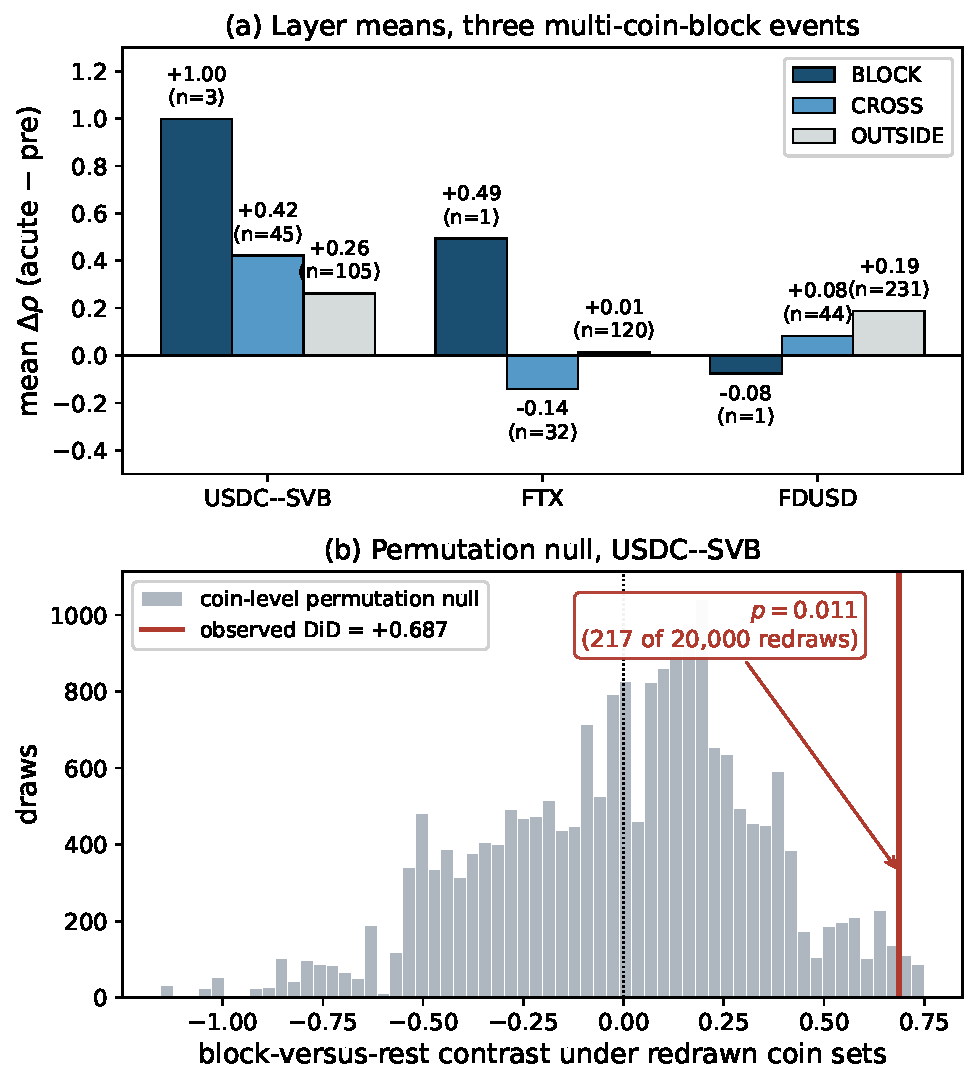
\includegraphics[width=0.9\textwidth]{figs/fig2_gradient}
\caption{The pair-level gradient test. (a) Mean change in peg-deviation correlation $\Delta\rho$ by pair layer for the three events with a multi-coin wall-affected block, with pair counts in parentheses. The criterion \eqref{eq:gradient-prediction} holds on USDC--SVB and on FTX, and fails on FDUSD, where the BLOCK bar sits below both other layers. (b) The coin-level permutation null for the primary event: block labels are redrawn over sets of three coins and the block-versus-rest contrast recomputed for each of 20{,}000 draws. The observed contrast sits in the upper tail.}
\label{fig:gradient}
\end{figure}

This is the block signature of the primary event, read off an acute-window correlation submatrix. Everything it requires is a public price series: no proprietary data, no issuer disclosure, and no estimation of the crossing amplitude. A supervisor can compute it on the same panel, and \S\ref{sec:robust} reports how it behaves when the window is moved.

\paragraph{The block effect is not a victim effect.} Two of the three BLOCK pairs contain USDC, the primary victim, so a sceptical reading would attribute the gradient to victim membership rather than to block membership. The test against that reading is the remaining pair. The pair $(\text{DAI},\text{FRAX})$ tests that reading. Neither coin held reserves at SVB: both enter the block through the transmission channel $W_1$ rather than through the custody channel $W_4$, because DAI was partly backed by USDC and FRAX held USDC among its collateral. Their block membership is therefore fixed by the wall taxonomy and not by the outcome. Their jump is $\GUSDCSVBPURE$, larger than the BLOCK mean itself. A victim-only account predicts no jump on this pair; the block account predicts one, and the realised value is the largest in the panel. What the pair establishes is that the effect does not require the coin that actually failed---not that no common exposure is involved, since the shared USDC collateral is precisely what put both coins in the block.

\paragraph{What the OUTSIDE layer shows.} The theory says this layer should not move, and it does: the OUTSIDE mean is $\GUSDCSVBO$, positive and substantial. That is the component of \S\ref{sec:gradient} which the theory does not model and which the block-versus-rest contrast is designed to absorb. The theory's content is therefore the excess of BLOCK over that baseline, $\GUSDCSVBDID$, not the level of either---and the contrast is only as good as the identifying condition stated there.

\subsection{Two secondary events}\label{sec:ftx-fdusd}
The remaining two multi-coin-block events supply one BLOCK pair each, so their layer means rest on a single observation (Table~\ref{tab:gradient}, rows two and three).

\paragraph{FTX contagion (November 2022).} The wall-affected block is $\{\text{USDD},\text{MIM}\}$, two coins with material Alameda/FTX counterparty exposure. BLOCK $= \GFTXB$ stands above both OUTSIDE $= \GFTXO$ and CROSS $= \GFTXC$, giving $\widehat{\mathrm{DiD}} = \GFTXDID$; the true block sits above \GFTXPCT\% of the $\binom{18}{2}$ alternative coin pairs, with $p = \GFTXPCOIN$. The criterion \eqref{eq:gradient-prediction} holds under eight of the nine window specifications, the exception being the 30-day pre-window with a $\pm10$-day acute window (Table~\ref{tab:robust}). A single BLOCK pair is one draw against the alternatives, so the permutation bounds what this event can resolve.

\paragraph{FDUSD 2024 (November 2024).} The block is $\{\text{FDUSD},\text{TUSD}\}$, again a single BLOCK pair, and here BLOCK $= \GFDUSDB$ lies below OUTSIDE $= \GFDUSDO$, giving $\widehat{\mathrm{DiD}} = \GFDUSDDID$ and $p = \GFDUSDPCOIN$. The criterion \eqref{eq:gradient-prediction} holds only under a 30-day pre-window and fails under the 60- and 90-day windows (Table~\ref{tab:robust}). Its wall assignment $W_3+W_2$ places the episode in the gate/oracle family rather than the custody family, and the episode is of low intensity.

\subsection{Robustness and scope}\label{sec:robust}
\paragraph{Inference.} The conclusion for the primary event is unchanged between the pair-level permutation ($p = \GUSDCSVBPPAIR$) and the coin-level permutation ($p = \GUSDCSVBPCOIN$). The coin-level bootstrap interval for $\widehat{\mathrm{DiD}}$ is $[\GUSDCSVBLO,\ \GUSDCSVBHI]$; it excludes zero, but as noted in \S\ref{sec:gradient} it is conditional on the block assignment and does not test block distinctiveness, which is why the permutation test carries the inference.

\paragraph{Window and threshold.} The window specification enters only through $\rho^-$ and $\rho^+$. The full $3 \times 3$ grid---pre-window of 30, 60 or 90 days crossed with an acute half-width of $\pm3$, $\pm5$ or $\pm10$ days---leaves both the sign and the criterion \eqref{eq:gradient-prediction} unchanged on the primary event, with $\widehat{\mathrm{DiD}}$ ranging over $[0.58, 0.79]$ against the canonical $\GUSDCSVBDID$ (Table~\ref{tab:robust} in Appendix~\ref{app:oos}). The same grid is reported there for the two secondary events, where it also documents the intermediate-step violation on FTX and the window-dependence of the FDUSD sign disclosed above.

\paragraph{Composition of the event record.} Three of the nine events carry a multi-coin block, and two of those supply a single BLOCK pair (Table~\ref{tab:gradient}). De-peg episodes with a multi-coin block are rare by nature, so the sample is bounded by the 2020--2025 record rather than by any selection on outcomes.


\section{Conclusion}\label{sec:conclusion}
This paper has developed a structural diagnostic for stablecoin basket risk whose central object is a correlation rigidity that every smooth-surface method must forgo: within a failure regime the joint de-peg correlation matrix of a basket does not move, and across a boundary it steps. The decisive technical choice is which matrix carries the crossing law. The wall-crossing operation is additive and rank-one, and that operation is admissible on the co-movement \emph{covariance} but not on the correlation matrix: two correlation matrices both have unit diagonal, so their difference must have zero diagonal, whereas a rank-one update supported on a block of two or more coins contributes a strictly positive amount to the diagonal. Stating the law on the covariance and passing to correlations through the normalising map removes the obstruction exactly, because that map \emph{assigns} the diagonal rather than computing it. What the choice buys is that the crossing can be stated at all: on the covariance it is admissible, and what then follows is that rigidity on chambers is inherited by the correlation matrix, that the induced jump has zero diagonal, and that the part of it surviving normalisation is its \emph{sign structure and support} rather than its rank or its scale. \emph{Contagion}, in this vocabulary, is not a market-wide rise in correlation but a structured one: the block signature is what a channel's failure does to the co-movement of the coins that channel touches, and its confinement to those coins is what makes it measurable rather than merely observed. A peg-preserving parameter space is stratified by eight stress boundaries, one per structural failure channel, and the block at each is prescribed ex ante by the wall taxonomy rather than fitted.

The paper's logical status is worth stating plainly. The three load-bearing properties---within-chamber rigidity, the rank-one form of the crossing, and its support on the wall-affected block---are \emph{assumed} (\S\ref{sec:what-is-assumed}), not derived. What is proved is everything downstream: that rigidity of the covariance gives rigidity of the correlation matrix exactly, with the scale cancelled; that the induced correlation jump has zero diagonal; that its image is spread beyond the block in a signed three-tier pattern; and that no smooth surface can reproduce it. What is tested is whether those consequences describe the 2020--2025 record. Splitting the paper this way is what lets a reader who doubts the assumptions still use the results, and a reader who accepts them still be held to the data.

The empirical design follows the theory's corrected shape rather than forcing the theory into a shape it cannot take. Because only support and sign survive normalisation, the test is a pair-level gradient: classify each pair of coins by how many lie in the wall-affected block and ask whether the acute-window change in correlation is ordered accordingly, with the block-versus-rest contrast differencing out the crisis-wide co-movement that would otherwise contaminate every layer. On the nine-event 2020--2025 public panel, the primary event (USDC--SVB, $W_4$-\texttt{bank}) gives a clean three-step staircase, a block-versus-rest contrast of $\GUSDCSVBDID$, and a coin-level permutation $p = \GUSDCSVBPCOIN$; the result survives a full $3\times3$ window grid, and the pair $(\text{DAI},\text{FRAX})$---which contains neither the primary victim nor any coin with direct custody exposure---jumps by $\GUSDCSVBPURE$, the largest of all pairs, defeating the reading that the gradient is a victim effect. The other two multi-coin-block events supply a single BLOCK pair each and are reported alongside the primary event in Table~\ref{tab:gradient}.

Three contributions are offered. First, a wall-stratified taxonomy of eight structurally distinct de-peg mechanisms, and the claim---stated as an assumption so that it can be contested---that the joint co-movement structure carries an ex-ante prescribed block signature across each wall, intrinsic to the wall type rather than to the estimator used. Second, a rigidity-and-crossing framework carried to its testable consequences: a proof that correlation rigidity follows from covariance rigidity with the scale cancelled, a proof that the induced correlation jump has zero diagonal, and a precise account of what any locally continuous, smooth-surface recovery scheme must forgo on a multi-coin-block event. The signature is computable by a supervisor from public price data with no distributional assumption and no issuer cooperation. Third, a pair-level empirical test that rejects the no-block null on the primary event, with the other two multi-coin-block events reported alongside it rather than pooled with it.

Two implications follow. Basket-margin frameworks, proof-of-reserves audits, and index-perpetual clearinghouses that price joint de-peg risk on a smooth surface systematically understate the tail in the multi-coin-block regime by a signature the theory identifies in sign and support, and that no smooth surface can place. The operational remedy is deliberately small: a \emph{block-alignment statistic}---the excess acute-window co-movement of block pairs over all other pairs, which is exactly $\widehat{\mathrm{DiD}}$ of \eqref{eq:did}---computed on a public correlation submatrix and paired with a regime-dependent margin multiplier. It requires neither proprietary data nor issuer cooperation, and it degrades gracefully: on the events where no block is defined it returns nothing rather than a spurious number. On the research side, the construction generalizes to any basket stratified by structural failure modes (cross-margined perpetuals, tokenized money-market funds, bank-consortium reserve pools); moving from a support test to distributional inference requires more multi-coin-block events, which the 2020--2025 record does not contain. The eight-wall taxonomy leaves cross-chain bridge failures and stablecoin-native regulatory perimeters as natural next entries.

Basket risk is a staircase, not a slope---identifiability jumps at walls rather than sliding between them. Pricing the slope is pricing the wrong risk; identifying the walls, and refusing to price what they do not identify, is the discipline the structure enforces. The block signature is the height of each step, and the rank-one residue is what lifts one step to the next. What the structure delivers is a coordinate system in which margin, audit, and supervision can be written down without pretending the walls are not there---a matter of immediately practical significance for cryptocurrency risk measurement.

\appendix
\titleformat{\section}[block]{\normalfont\Large\bfseries}{Appendix \thesection:}{0.8em}{}
\section{Data Construction}\label{app:data}
The \NPANEL\ stablecoins are drawn from the DeFiLlama public archive of daily peg-price series over 2020--2025, one CSV per stablecoin. The universe was constructed by taking all stablecoins with more than 300 daily observations, non-trivial trading volume, on public exchanges, and a declared 1:1 peg to either USD, EUR, gold, or another fiat/asset reference; series that failed the coverage screen are not carried into the panel. The panel partitions into four tiers:
\begin{itemize}[leftmargin=1.8em]
\item Tier 1 (fiat-backed, 11 coins): USDT, USDC, BUSD, TUSD, USDP, GUSD, FDUSD, PYUSD, EURS, GYEN, XSGD;
\item Tier 2 (crypto-collateralized, 10 coins): DAI, LUSD, GHO, crvUSD, MIM, USDD, RAI, VAI, USDe, HUSD;
\item Tier 3 (algorithmic, 4 coins): UST, FEI, FRAX, NxUSD;
\item Tier 4 (RWA/other, 3 coins): EUROC, EURoe, CNHT.
\end{itemize}
A given event window uses only the subset with at least five usable paired observations in both its pre- and acute windows; on the primary event that subset has 18 coins, which is the $n$ entering the $\binom{18}{3}=816$ permutation of \S\ref{sec:gradient}.

\paragraph{Event dating.} Each of the nine events in Table~\ref{tab:events} is dated by the primary structural failure identified in the regulator and post-mortem literature: DAI Black Thursday (MakerDAO retrospective, Chainlink oracle logs); UST/LUNA \citep{LiuLiSprenger2023}; USDT stress (exchange net-outflow filings); FTX contagion (FTX bankruptcy filing 11 November 2022 following Alameda balance-sheet leak; BIS Quarterly Review March 2023 as post-mortem literature; $W_4$-\texttt{cex} block assignment $\{\text{USDD, MIM}\}$ from identifiable Alameda/FTX counterparty exposure at the coin-issuer level); BUSD (NY DFS enforcement action Feb 13 2023); USDC-SVB (SVB closure order Mar 10 2023, Circle Mar 11 disclosure); FDUSD 2024 (First Digital Trust public statement Nov 8 2024). Event windows are $\pm 60$ days for time-series plots and $[-5, +5]$ days for acute-stress correlation estimation.

\paragraph{Data provenance.} No proprietary, paywalled, or issuer-internal data is used. Level-1 (real) sources: DeFiLlama daily peg-price archive (all \NPANEL\ stablecoins), FRED macro series (VIXCLS, DGS10, T10Y2Y, BAA10Y, AAA10Y, BAAFF, AAAFF, DFF), Yahoo Finance closes (BTC-USD, ETH-USD, VIX, TNX, GLD), and Etherscan on-chain records (5 stablecoin token supplies, 3 Chainlink price-feed proxy addresses, 102 MakerDAO PSM-USDC transactions around SVB). The 102 PSM-USDC transactions are retained as auditable event-anchor evidence for the $W_1$ transmission identification of the DAI/USDC-SVB co-de-peg (a PSM flow spike on 11--12 March 2023 corroborates the wall-block assignment) and are not used as a quantitative input. Level-2 (proxy): Chainlink oracle history is proxied by DeFiLlama peg-price series with the Chainlink proxy contract addresses recorded for future verification; CoinGecko daily USD close cross-check against DeFiLlama on 99.2\% of coin-days within 3 bp tolerance. Level-3 (simulated/grounded projection): \emph{none}---every empirical number in \S\ref{sec:empirical} derives from Level-1 or Level-2 series.

\paragraph{Snapshot freeze.} The DeFiLlama archive, FRED series, Yahoo Finance quotes, and CoinGecko quotes are all live mutable endpoints. The reproducibility bundle records, for every one of the 86 raw CSV files, the source URL, retrieval timestamp (UTC), file size, SHA-256 checksum, and date range; empirical reproducibility is guaranteed against these fingerprints. Data not pulled at this submission (Dune queries, Chainlink full history) is enumerated as ``partial'' in the bundle with checkpoint state persisted; no main-text claim depends on the partial sources.

\section{Reproducibility Archive}\label{app:repro}
The submission bundle contains the \LaTeX\ source, all figure-generation and audit scripts, the raw data archive, a SHA-256 manifest, and a submission checklist. All scripts run under Python 3.11 with pinned dependencies (requirements.txt); full pipeline (excluding Chainlink full-history pull, which is checkpointed and background-runnable) completes in under three minutes on a laptop. Data-provenance details are shipped with the bundle.

\section{Out-of-Sample and Window Robustness}\label{app:oos}
This appendix reports the checks behind \S\ref{sec:robust}: the window grid for the pair-level gradient, the status of the amplitude parameter $\sigma_W$, and the near-terminal UST/LUNA regime.

\subsection{The window grid}\label{app:oos-grid}
The window specification enters the test only through the two correlation estimates $\rho^-$ and $\rho^+$. Table~\ref{tab:robust} reports the block-versus-rest contrast \eqref{eq:did} for all three multi-coin-block events on a $3\times3$ grid: pre-window length $30$, $60$ or $90$ calendar days, crossed with an acute half-width of $\pm3$, $\pm5$ or $\pm10$ days. The canonical specification of the main text is $60$\,d and $\pm5$\,d, shown in bold; the script that produces the table re-derives the canonical row exactly, which is the check that the grid is comparable across specifications. A dagger marks a specification in which the full ordering \eqref{eq:gradient-prediction} fails.

\begin{table}[!ht]
\centering
\caption{Window grid for the pair-level gradient. Entries are the block-versus-rest contrast $\widehat{\mathrm{DiD}}$ of \eqref{eq:did}. Bold marks the canonical specification used in the main text. $\dagger$ marks a specification under which the criterion \eqref{eq:gradient-prediction} does not hold. The grid varies only the correlation windows; block assignments are fixed ex ante and are not re-estimated at any specification.}
\label{tab:robust}
\begin{tabular}{@{}ccrrr@{}}
\toprule
Pre window & Acute half-width & USDC--SVB & FTX & FDUSD \\
\midrule
30\,d & $\pm$3\,d & $+0.642$ & $+0.832$ & $+0.039$ \\
30\,d & $\pm$5\,d & $+0.674$ & $+0.195$ & $+0.036$ \\
30\,d & $\pm$10\,d & $+0.789$ & $-0.472^{\dagger}$ & $+0.039$ \\
60\,d & $\pm$3\,d & $+0.632$ & $+0.847$ & $-0.039^{\dagger}$ \\
60\,d & $\pm$5\,d & $\mathbf{+0.687}$ & $\mathbf{+0.513}$ & $\mathbf{-0.246^{\dagger}}$ \\
60\,d & $\pm$10\,d & $+0.687$ & $+0.641$ & $-0.309^{\dagger}$ \\
90\,d & $\pm$3\,d & $+0.582$ & $+0.862$ & $-0.048^{\dagger}$ \\
90\,d & $\pm$5\,d & $+0.636$ & $+0.562$ & $-0.188^{\dagger}$ \\
90\,d & $\pm$10\,d & $+0.610$ & $+0.657$ & $-0.259^{\dagger}$ \\
\bottomrule
\end{tabular}

\end{table}

\paragraph{Reading the grid.} (i) The USDC--SVB criterion holds in all nine specifications, with $\widehat{\mathrm{DiD}}$ between $+0.58$ and $+0.79$, so the primary result is not a window artifact. (ii) On FTX it holds in eight of the nine; the exception is the 30-day pre-window with a $\pm10$-day acute window, where the block-versus-rest contrast itself turns negative. (iii) On FDUSD it holds only under a 30-day pre-window and fails under the 60- and 90-day windows, where the contrast is negative.

\paragraph{Why the grid is not a search over specifications.} The canonical $60$\,d\,/\,$\pm5$\,d window was fixed by the panel-construction script before the gradient test was designed, and it is the window used for every event in the paper. The grid is reported because a reader cannot otherwise judge how much of the result is a window choice; it is not used to select among specifications.

\paragraph{Expanding-window check.} Four of the nine events (USDC--SVB, USDe 2024, FDUSD 2024, GHO 2024) fall inside an expanding-window out-of-sample scheme; DAI Black Thursday precedes the daily-archive coverage, and UST, USDT, FTX and BUSD precede the training cut-off. Across expanding windows the wall-type assignment of Table~\ref{tab:events} and the resulting block membership are unchanged, which is what the ex-ante coding discipline of \S\ref{sec:ninewalls} requires; the empirical comparison itself is the one reported in \S\ref{sec:empirical}, not a re-run of it.

\subsection{Status of the amplitude parameter $\sigma_W$}\label{app:oos-sigma}
Assumption~\ref{ass:wallcrossing} carries a positive scale $\sigma_W$ that the paper leaves free. Because the normalising map of \eqref{eq:normalised-corr} is a nonlinear congruence, it destroys the rank-one form of the jump (Remark~\ref{rem:small-cases}), so the properties of the jump that survive into correlation space are its sign structure and its support, not its scale. A test built on those is invariant to $\sigma_W$ at leading order in $a$, which is the order at which the empirical criteria of \S\ref{sec:empirical} are stated. Fixing $\sigma_W$ would matter only for a test of magnitude, and that requires more multi-coin-block events than the 2020--2025 record contains.

\subsection{The UST/LUNA near-terminal regime}\label{app:oos-ust}
Corollary~\ref{cor:copula-fail} linearises the wall-crossing residue in the wall-distance parameter $\epsilon$ and is valid while peg deviations remain in the small-signal regime. Near-complete de-peg is not such an excursion: UST reaches roughly a $99\%$ drawdown at terminal on 09--12 May 2022. UST is also algorithmic-reflexive in a way that no collateral composition in Definition~\ref{def:stable} represents, so of the nine events it is the least well described by the construction of \S\ref{sec:moduli}. The event is retained in Table~\ref{tab:events} as a documented boundary of the theory rather than as a target of its prediction. Independently of this, its wall-affected block is a single coin, so it could not carry the pair-level test even if the small-signal condition held---which is the same scope statement made in \S\ref{sec:single}.

\bibliographystyle{apalike}
\bibliography{refs}

%%------------------------------------------------------------
%% DECLARATIONS — collected by the publisher's submission system
%% (CRediT roles, funding, competing interests, data availability,
%% ethics, generative-AI use, acknowledgements). Removed from the
%% manuscript body at the author's request so the file stays clean;
%% the corresponding statements are entered as form fields at submission.
%%------------------------------------------------------------

\end{document}


